\section{Zielsetzung}
\label{sec:Zielsetzung}

Im Versuch V703 soll die Kennlinie des Zählrohres, die Steigung des Geiger-Müller Plateaus und die Totzeit bestimmt werden.

\section{Theorie}
\label{sec:Theorie}

Das Geiger-Müller-Zählrohr ist ein Detektor für ionisierende Strahlung. 
Ionisierende Strahlung ist in α-, β- und γ-Strahlung unterteilt. 
α-Strahlung besteht aus Heliumkernen, β-Strahlung aus Elektronen und γ-Strahlung aus Photonen.
Das Geiger-Müller-Zählrohr ist am besten für die Messung von 
α- und γ-Strahlung geeignet. Die Nachweisbarkeit von γ-Strahlung ist klein.
\\
Das Zählrohr besteht aus aus einem Anodendraht und einer Kathodenhülle.
Zwischen Kathode und Anode wird eine Spannung angelegt.
Durch eine dünne Mylarfolie ist das Rohr verschlossen.
Im Inneren befindet sich ein Gasgemisch aus Argon und einem Alkohol.
Durch eintretende Strahlung wird Argon ionisiert. 
Aufgrund das E-Feld im Inneren werden die Gasionen zum Kathodenzylinder und die Elektronen zum Anodendraht hin beschleunigt.
Die freigesetzten Elektronen können auf ihrem Weg zur Kathode in einer Kettenreaktion weitere Ion-Elektron-Paare erzeugen.
Über diesen Prozess wird ein Stromfluss erzeugt, welcher jedoch schnell wieder über den Widerstand im $\si{\m\O}$-Bereich abfällt.
So bald die Ladungsträger wieder abgeflossen sind baut sich das E-Feld im inneren des Zählrohrs wieder auf.
\\
Aufgrund der geringen Stärke der Spannungsimpulse, müssen sie mithilfe eines Versärkers 
für den angeschlossenen Zähler verstärkt werden.
\\
\begin{figure}[h!]
    \centering
    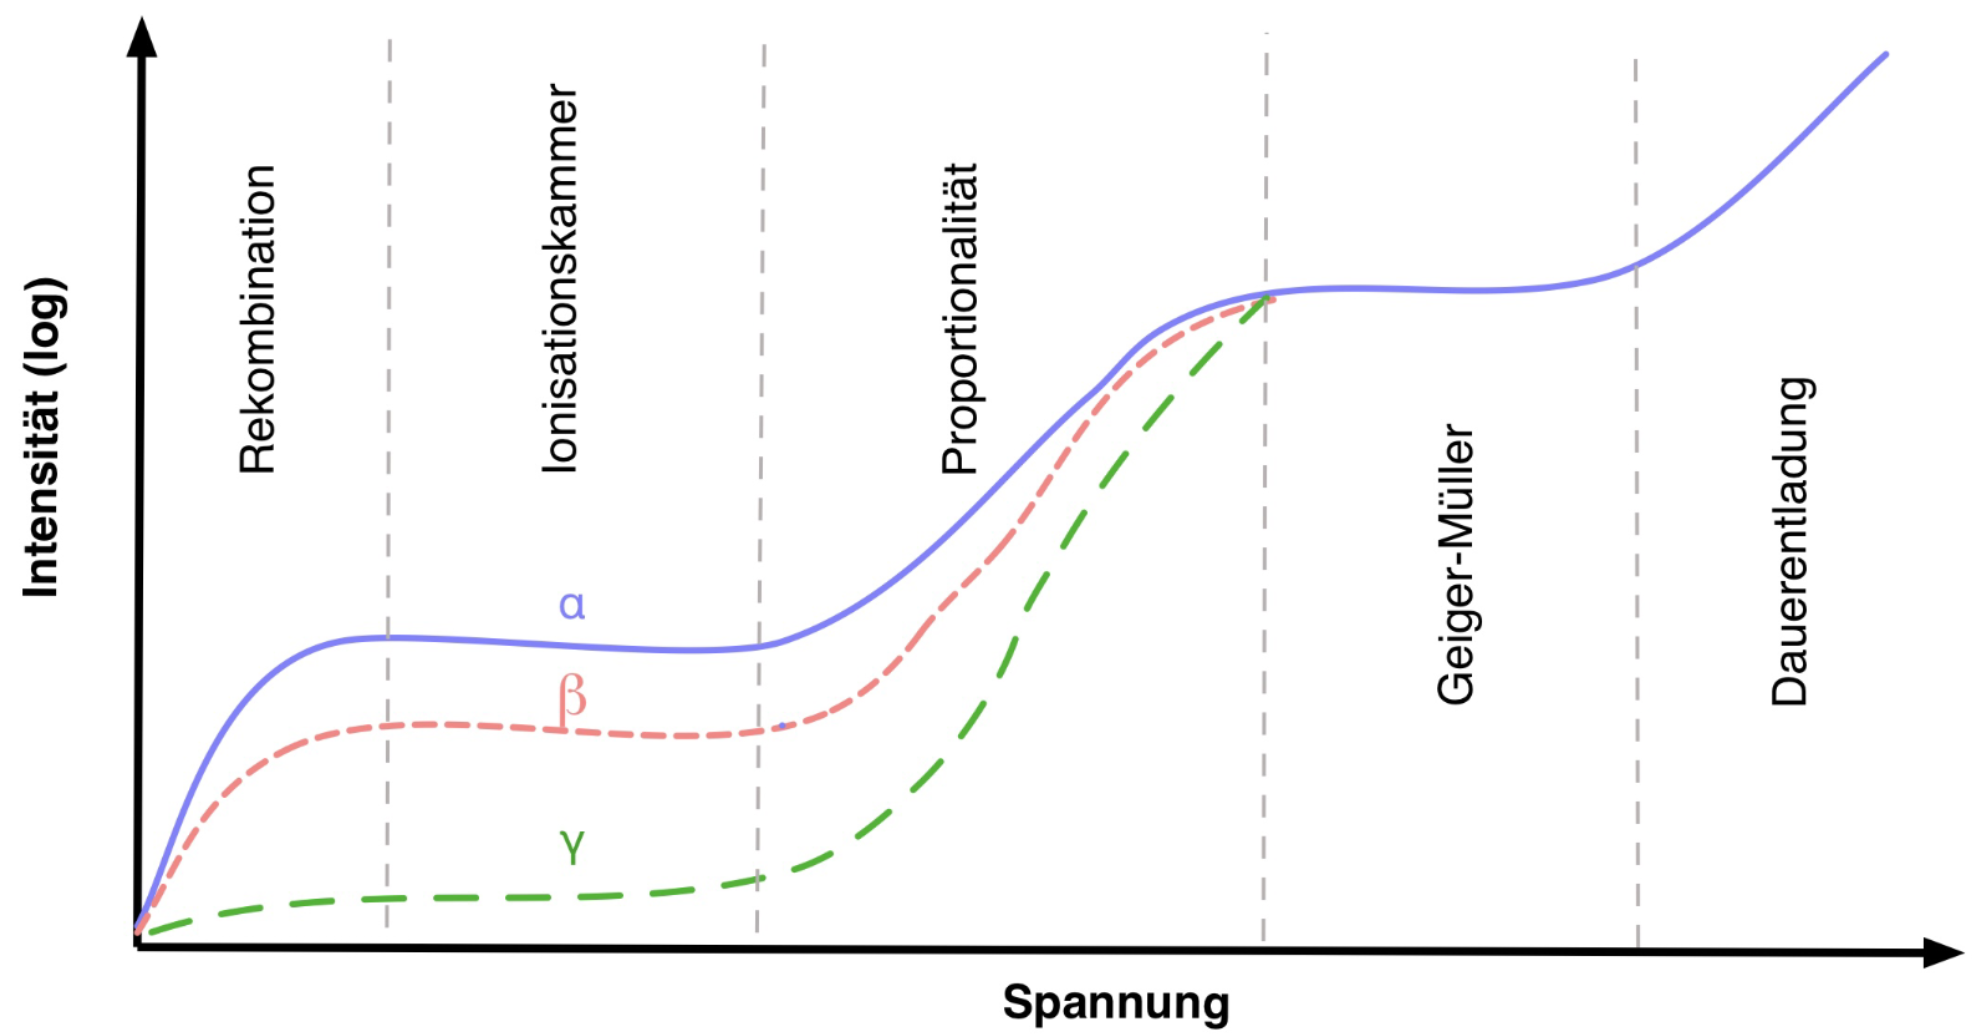
\includegraphics[width=0.5\textwidth]{img/gm-charakteristik.png}
    \caption{Charakteristische Bereiche des Geiger-Müller-Zählrohrs.\cite{V703}}
    \label{fig:gm-charakteristik}
\end{figure}
\\
Das Detektierverhalten des Geiger-Müller-Zählrohrs ist abhängig von der angeschlossenen Spannung.
Die Interaktion mit Strahlung lässt sich, wie in der \autoref{fig:gm-charakteristik} zu sehen, in mehrere Bereiche aufteilen.
Im ersten Bereich, der Rekombination, verbinden sich Gasionen und Elektronen 
mehrheitlich bevor sie die Kathode, beziehuungsweise die Anode erreichen. 
\\
\\
Im Bereich \textbf{Ionisationskammer} verhält sich das Zählrohr wie eine Ionisationskammer.
Es kommt zu einem vernachlässigbar geringen Menge an Rekombination.
Es werden nur Ladungen detekiert, die durch die eingehende Strahlung getrennt werden.
\\
\\
Im \textbf{Proportionalitätsbereich} werden Ladungspaare auch durch freie Elektronen erzeugt.
Die große Feldstärke in der Nähe des Drates lößt Townsend-Lawinen aus. Dabei werden örtlich begrenzt hohe Mengen an Elektronen freigesetzt.
Abhängig von Spannung, Gasart und Gasdruck kommt es zu einer Verstärkung des Strahlungsimpulses.%?????
$α$-Teilchen erzeugen in diesem Bereich eine deutlich größere Ladung als $β$- und $γ$-Teilchen.
Dadurch ist es möglich die Strahlungsarten zu unterscheiden.
\\
\\
Im \textbf{Geiger-Müller-Bereich} werden zusätzlich noch Gasatome angeregt.
Diese emmitieren daraufhin Photonen, welche Photoelektronen freisetzen.
Auch durch diesen Prozess entstehen Elektronenlawinen.
Dieser Effekt kann durch die Zugabe von Alkoholgas unterdrückt werden.
Die Photonen werden durch den Alkohol absorbiert. Im Gegensatz zum Proportionalitätsbereich,
sind die Townsend-Lawinen nicht mehr lokal begrenzt. Die frei werdenden Elektronen fließen über die Kathode ab.
Die Gasionen sind träge und sammeln sich um die Anode herum und begrenzen dadurch die Ausbildung weiterer Lawinen.
Die Größe der entstehenden Impulse ist unabhängig von der Art der einfallenden Strahlung.
Der Geiger-Müller-Bereich ist der Arbeitsbereich des Zählrohrs. 
Eine Erhöhung der Spannung führt nur zu einer geringfügigen Steigerung der Detektionsrate.
In diesem Geiger-Müller Plateau wird in das erste Drittel der Arbeitspunkt gelegt.
Dieser gibt die Betriebsspannung des Zählrohrs an.\\
\\
Steigert man die Spannung weiter, so kommt es zu einer \textbf{Dauerentladung}.
Die Detektionsrate steigt stark an. Dieser Zustand ist schädlich für die Apparatur.
\\
\\
Weitere Effekte die beachtet werden müssen. Beim auftreffen der Ionen auf die Kathode,
können weitere Elektronen freigesetzt werden. Diese können zeitlich versetzt weitere Impulse erzeugen.
Die Wahrscheinlichkeit einer solchen Nachentladung nimmt mit steigendem Verschleiß des Detektors und höherer Spannung zu.
Das Geiger-Müller Plateau hat deswegen eine Steigung s.
\begin{equation*}
    s = \frac{ΔN}{N} \cdot 100\%/\SI{100}{\volt}.
\end{equation*}
Die Steigung wird aus der relativen Zählrateänderung bei einer Spannungsdifferenz von $\SI{100}{\volt}$ berechnet.
Durch die Steigung ist es möglich die Qualtität des Zählrohrs zu bestimmen.\\
\\
\\
\subsection{Totzeit}
\label{sec:Totzeit}

Haben sich alle freigesetzten Elektronen auf der Anode gesammelt, befinden sich nur noch Gasionen im Zählrohr.
Durch die ansammlung positiver Ladungen sinkt das E-Feld stark ab und es kann keine weitere Strahlung mehr detektiert werden.
Dieser Zustand wird Totzeit genannt. So bald die Ladung wieder abgegeben wurde, baut sich das E-Feld wieder auf und das Geiger-Müller-Zählrohr ist wieder betriebsbereit.
Auf die Totzeit folg die Erholungszeit, in der zwar Strahlung detektiert werden kann, jedoch die Zählrohrspannung noch nicht wieder ihre volle Stärke erreicht hat.
\\
Zur Bestimmung der Totzeit kann die Zwei-Quellen-Methode verwendet werden.
Bei dieser wird davon ausgegangen, dass mit steigender Zählrate die Zählratenverluste durch die Totzeit $τ$ zunimmt.
Die tatsächliche Zählrate $N_0$ lässt sich mithilfe der gemessenen Zählrate $N$ und der Totzeit $τ$ berechnen.
\begin{equation*}
    N_0 = \frac{N}{1-N \cdot τ}.
\end{equation*}
Der aus der Totzeit resultierende Zählratenverlust kann berechnet werden mit
\begin{equation*}
    N_0 - N = \frac{N^2 \cdot τ}{1 - N \cdot τ}.
\end{equation*}
Misst man die Zählrate zweier Quellen zuerst getrennt und dann kombiniert, lässt sich die Totzeit mit
\begin{equation}\label{eq:totzeit}
    τ = \frac{N_1 + N_2 - N_{12}}{N_{12}^2 - N_1^2 - N_2^2}
\end{equation}
berechnen.
\\
\\
\subsection{Messunsicherheit}
\label{sec:Messunsicherheit}
Der relative Fehler einer Größe, die der Poissonverteilung unterliegt, lässt sich mit
\begin{equation}
    \frac{\sqrt{N}}{N} = \frac{1}{\sqrt{N}}
\end{equation}
berechnen. Hierbei ist $N$ die Anzahl der Ereignisse. Der absolute Fehler ist also $\sqrt{N}$.
